\documentclass[11pt]{article}
\usepackage[a4paper,margin=1in]{geometry}
\usepackage{enumitem}
\usepackage{titlesec}
\usepackage{fancyhdr}
\usepackage{graphicx}
\usepackage{xcolor}
\usepackage{tcolorbox}
\usepackage{booktabs}
\usepackage{longtable}
\usepackage{listings}
\usepackage[T1]{fontenc}
\usepackage{hyperref}

\definecolor{mainblue}{RGB}{0,70,140}
\definecolor{lightblue}{RGB}{235,245,255}
\hypersetup{colorlinks=true,linkcolor=mainblue,urlcolor=mainblue}

\lstset{
    basicstyle=\ttfamily\small,
    backgroundcolor=\color{gray!10},
    frame=single,
    breaklines=true,
    columns=fullflexible,
    keywordstyle=\color{mainblue},
    commentstyle=\color{gray}
}

\pagestyle{fancy}
\fancyhf{}
\lhead{\textcolor{mainblue}{Fundamentals of Accounting}}
\rhead{\textcolor{mainblue}{Small Business Accounting System}}
\rfoot{\textcolor{mainblue}{Page \thepage}}

\titleformat{\section}{\large\bfseries\color{mainblue}}{\thesection}{1em}{}
\titleformat{\subsection}{\normalsize\bfseries\color{mainblue}}{\thesubsection}{1em}{}
\titlespacing*{\section}{0pt}{12pt}{5pt}
\titlespacing*{\subsection}{0pt}{8pt}{3pt}
\setlength{\parskip}{5pt}
\setlength{\parindent}{0pt}

\begin{document}

%------------------------------------------------ title page
\begin{center}
\IfFileExists{NUCES.png}{\includegraphics[width=0.22\textwidth]{NUCES.png}\\[1em]}{\vspace*{2.2cm}}
\begin{tcolorbox}[colback=lightblue,colframe=mainblue,width=0.88\textwidth]
\centering
{\Large \textbf{Project Report}}\\[6pt]
{\large Small Business Accounting System}\\[6pt]
{\normalsize Fundamentals of Accounting \quad Class: BCS 9th}\\[4pt]
{\normalsize Course Instructor: Dr. Sami Ullah}
\end{tcolorbox}
\vspace{1.2em}
\textbf{Student Name:} Syed Khadeen \quad \textbf{Roll No:} 22P-9150\\[12pt]
\textbf{Submission date:} 20 November 2026
\end{center}

\newpage
\tableofcontents
\newpage

% ============================================================
\section{Introduction, Objectives, and Problem Statement}
% ============================================================

Small businesses that keep manual books are prone to arithmetic errors,
unbalanced entries, and slow report preparation. This project
implements the fundamental accounting cycle (from chart of accounts to
financial statements) as a small web application. It removes manual
calculation errors and gives the owner instant trial balance, income
statement, and balance sheet reports.

\subsection*{Objectives}
\begin{enumerate}[label=\arabic*.]
    \item Implement a chart of accounts covering assets, liabilities, equity, revenue, and expenses.
    \item Record transactions using double-entry bookkeeping, with system-level validation that every entry balances (debits = credits).
    \item Post entries automatically to a general ledger and compute running account balances.
    \item Generate an unadjusted trial balance.
    \item Produce an income statement and balance sheet derived directly from ledger balances, with no manual recalculation.
\end{enumerate}

\subsection*{Problem Statement}
Given a stream of raw business transactions, the system must produce
consistent, mathematically balanced financial statements with no
manual posting step.

% ============================================================
\section{System Requirements and Functional Specifications}
% ============================================================

\subsection*{Functional Requirements}

\begin{longtable}{p{0.5cm} p{6.5cm} p{6.5cm}}
\toprule
\textbf{\#} & \textbf{Requirement} & \textbf{Where implemented} \\
\midrule
\endhead
1 & Chart of accounts (cash, A/R, equipment, A/P, capital, revenue, expenses) & \texttt{app/seed.py} $\rightarrow$ \texttt{CHART\_OF\_ACCOUNTS}, "Chart of Accounts" page \\
2 & $\geq$15 transactions, double-entry & \texttt{app/seed.py} $\rightarrow$ \texttt{TRANSACTIONS} (18 entries) \\
3 & Journal entries with debit/credit amounts & \texttt{app/accounting.py::post\_entry}, "Record Transaction" / "Journal" pages \\
4 & Ledger accounts with balances & \texttt{app/accounting.py::get\_ledger}, "General Ledger" page \\
5 & Unadjusted trial balance & \texttt{app/accounting.py::get\_trial\_balance}, "Trial Balance" page \\
6 & Income statement and balance sheet & \texttt{get\_income\_statement} / \texttt{get\_balance\_sheet} \\
7 & Validate debits = credits per entry & \texttt{post\_entry} raises \texttt{UnbalancedEntryError} if not equal \\
\bottomrule
\end{longtable}

\subsection*{Non-functional Requirements}
\begin{itemize}
    \item Runs locally, no internet dependency (SQLite file database).
    \item Single-user desktop/browser application (Streamlit).
    \item Reports exportable to CSV for printing/submission.
\end{itemize}

\subsection*{Technology Stack}
\begin{itemize}
    \item Python 3.10+
    \item Streamlit (UI)
    \item SQLite (storage, via Python's built-in \texttt{sqlite3})
    \item pandas (tabular display)
\end{itemize}

% ============================================================
\section{System Design / Architecture}
% ============================================================

\begin{figure}[h!]
    \centering
    \includegraphics[width=0.85\textwidth]{sys-arch-acc.jpg}
    \caption{System architecture: Streamlit UI $\rightarrow$ accounting engine $\rightarrow$ SQLite data access $\rightarrow$ database file.}
\end{figure}

\subsection*{Processing Flow (Accounting Cycle)}

\begin{figure}[h!]
    \centering
    \includegraphics[width=0.85\textwidth]{proc-flow-acc.jpg}
    \caption{Processing flow: business event $\rightarrow$ journal entry $\rightarrow$ validation $\rightarrow$ ledger $\rightarrow$ trial balance $\rightarrow$ financial statements.}
\end{figure}

% ============================================================
\section{Database Design (ER Diagram)}
% ============================================================

\begin{figure}[h!]
    \centering
    \includegraphics[width=0.85\textwidth]{erd-acc.jpg}
    \caption{ER diagram: accounts, journal\_entries, journal\_lines.}
\end{figure}

\begin{itemize}
    \item \texttt{accounts} to \texttt{journal\_lines}: one account, many postings (1:N).
    \item \texttt{journal\_entries} to \texttt{journal\_lines}: one entry, two or more balanced lines (1:N).
    \item Check constraints enforce \texttt{debit >= 0}, \texttt{credit >= 0}, and a line cannot be both a debit and a credit simultaneously.
\end{itemize}

% ============================================================
\section{Accounting Procedures and Transaction Examples}
% ============================================================

\subsection*{Chart of Accounts Used (13 accounts)}

\begin{longtable}{l l l l}
\toprule
\textbf{Code} & \textbf{Account} & \textbf{Type} & \textbf{Normal Balance} \\
\midrule
\endhead
1010 & Cash & Asset & Debit \\
1020 & Accounts Receivable & Asset & Debit \\
1030 & Supplies & Asset & Debit \\
1040 & Equipment & Asset & Debit \\
2010 & Accounts Payable & Liability & Credit \\
2020 & Notes Payable & Liability & Credit \\
3010 & Owner's Capital & Equity & Credit \\
3020 & Owner's Drawings & Equity & Debit \\
4010 & Service Revenue & Revenue & Credit \\
5010 & Rent Expense & Expense & Debit \\
5020 & Salaries Expense & Expense & Debit \\
5030 & Utilities Expense & Expense & Debit \\
5040 & Advertising Expense & Expense & Debit \\
\bottomrule
\end{longtable}

\subsection*{Sample Transactions (18 total, double-entry)}
Full list in \texttt{app/seed.py}; first five shown here as a worked example:

\begin{longtable}{l p{5.5cm} l l}
\toprule
\textbf{Date} & \textbf{Description} & \textbf{Debit} & \textbf{Credit} \\
\midrule
\endhead
2026-11-01 & Owner invested cash to start the business & Cash 50,000 & Owner's Capital 50,000 \\
2026-11-01 & Purchased equipment for cash & Equipment 12,000 & Cash 12,000 \\
2026-11-02 & Purchased supplies on account & Supplies 3,000 & Accounts Payable 3,000 \\
2026-11-03 & Borrowed cash from bank & Cash 15,000 & Notes Payable 15,000 \\
2026-11-04 & Billed client for services on account & Accounts Receivable 8,000 & Service Revenue 8,000 \\
\bottomrule
\end{longtable}

\subsection*{Accounting Equation Check}
Every transaction above keeps Assets = Liabilities + Equity in
balance, since each entry posts equal debit and credit amounts.

\subsection*{Validation Logic}
From \texttt{post\_entry} in \texttt{app/accounting.py}:

\begin{lstlisting}[language=Python]
total_debit = round(sum(l.get("debit", 0) for l in lines), 2)
total_credit = round(sum(l.get("credit", 0) for l in lines), 2)
if total_debit != total_credit:
    raise UnbalancedEntryError(...)
\end{lstlisting}

If a user submits an unbalanced entry through the UI, it is rejected
before it reaches the database. The trial balance can never go out of
balance because of a bad entry.

\subsection*{Ledger Posting}
For each account, running balance is calculated by adding debits and
subtracting credits (for debit-normal accounts), or the reverse (for
credit-normal accounts).

\subsection*{Trial Balance}
Sums each account's ending ledger balance into a debit or credit
column based on its normal balance; totals must match.

\subsection*{Income Statement}
Net Income = Total Revenue $-$ Total Expenses.

\subsection*{Balance Sheet}
Total Equity = Owner's Capital $-$ Drawings + Net Income; Total Assets
must equal Total Liabilities + Total Equity.

% ============================================================
\section{Screenshots and Explanation of Software Features}
% ============================================================

Screenshots are stored in \texttt{screenshots/}.

\begin{figure}[h!]
    \centering
    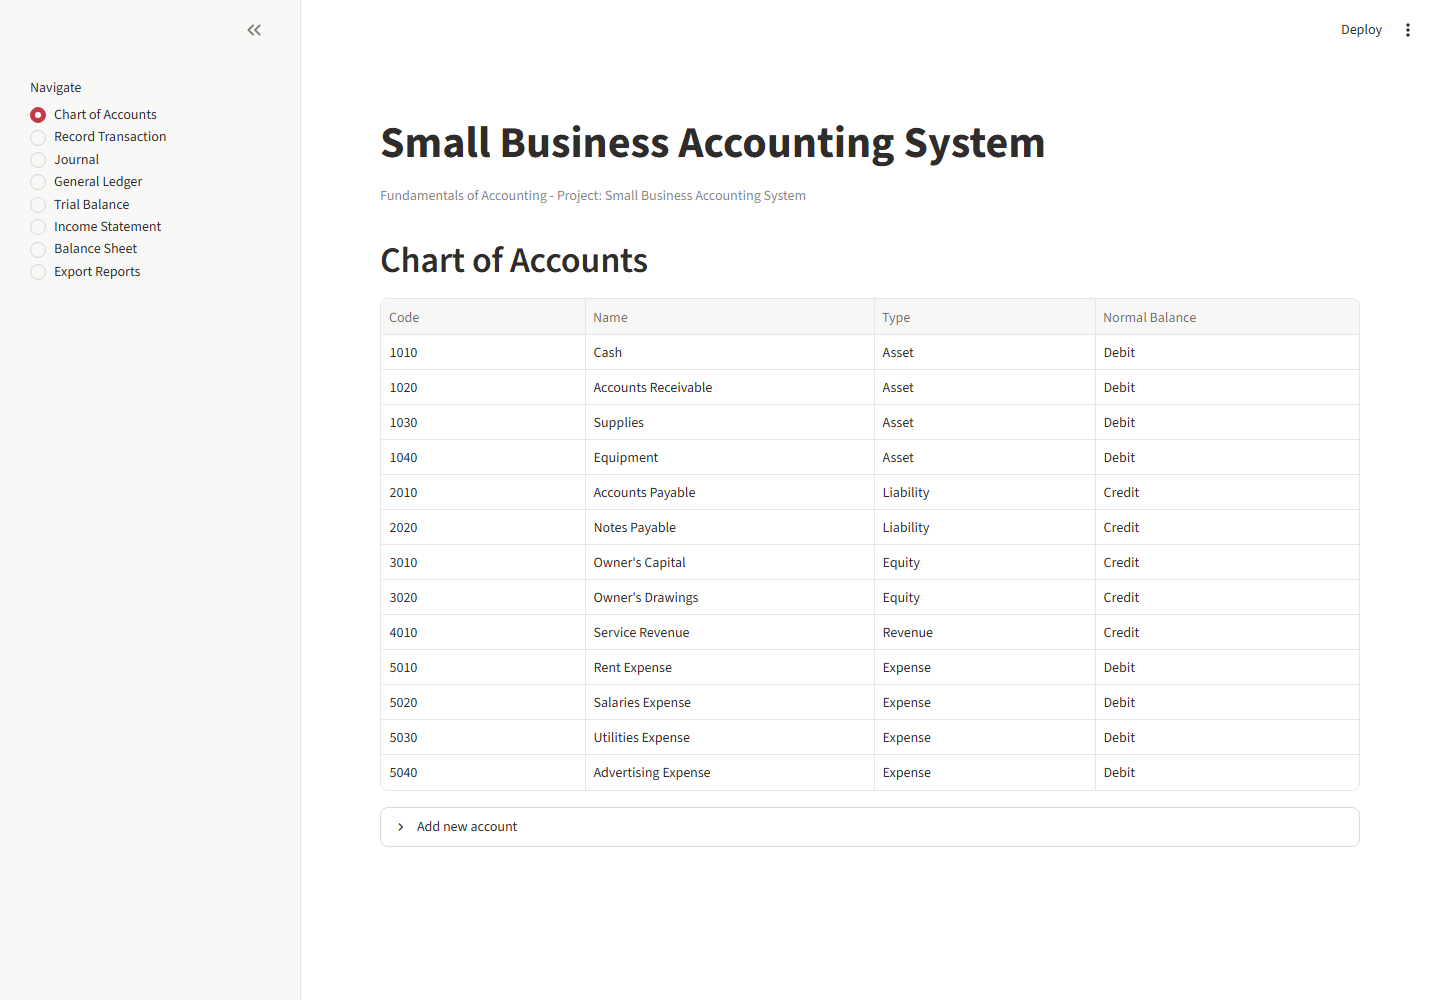
\includegraphics[width=0.85\textwidth]{../screenshots/01_chart_of_accounts.png}
    \caption{Chart of accounts table and "add account" form.}
\end{figure}

\begin{figure}[h!]
    \centering
    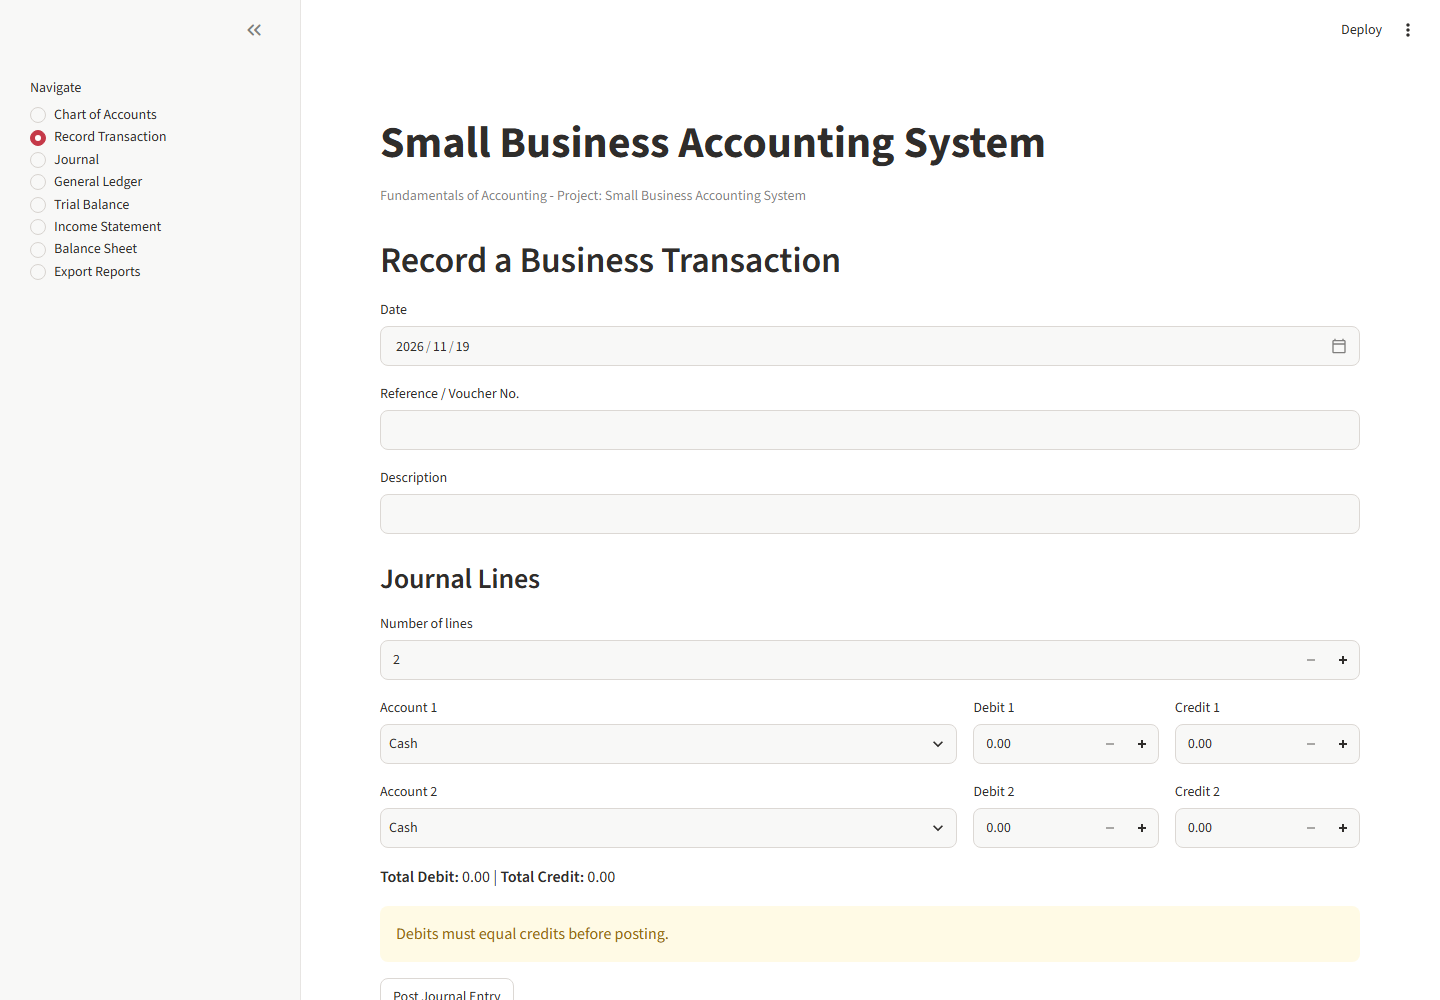
\includegraphics[width=0.85\textwidth]{../screenshots/02_record_transaction.png}
    \caption{Journal entry form with live debit/credit balance check.}
\end{figure}

\begin{figure}[h!]
    \centering
    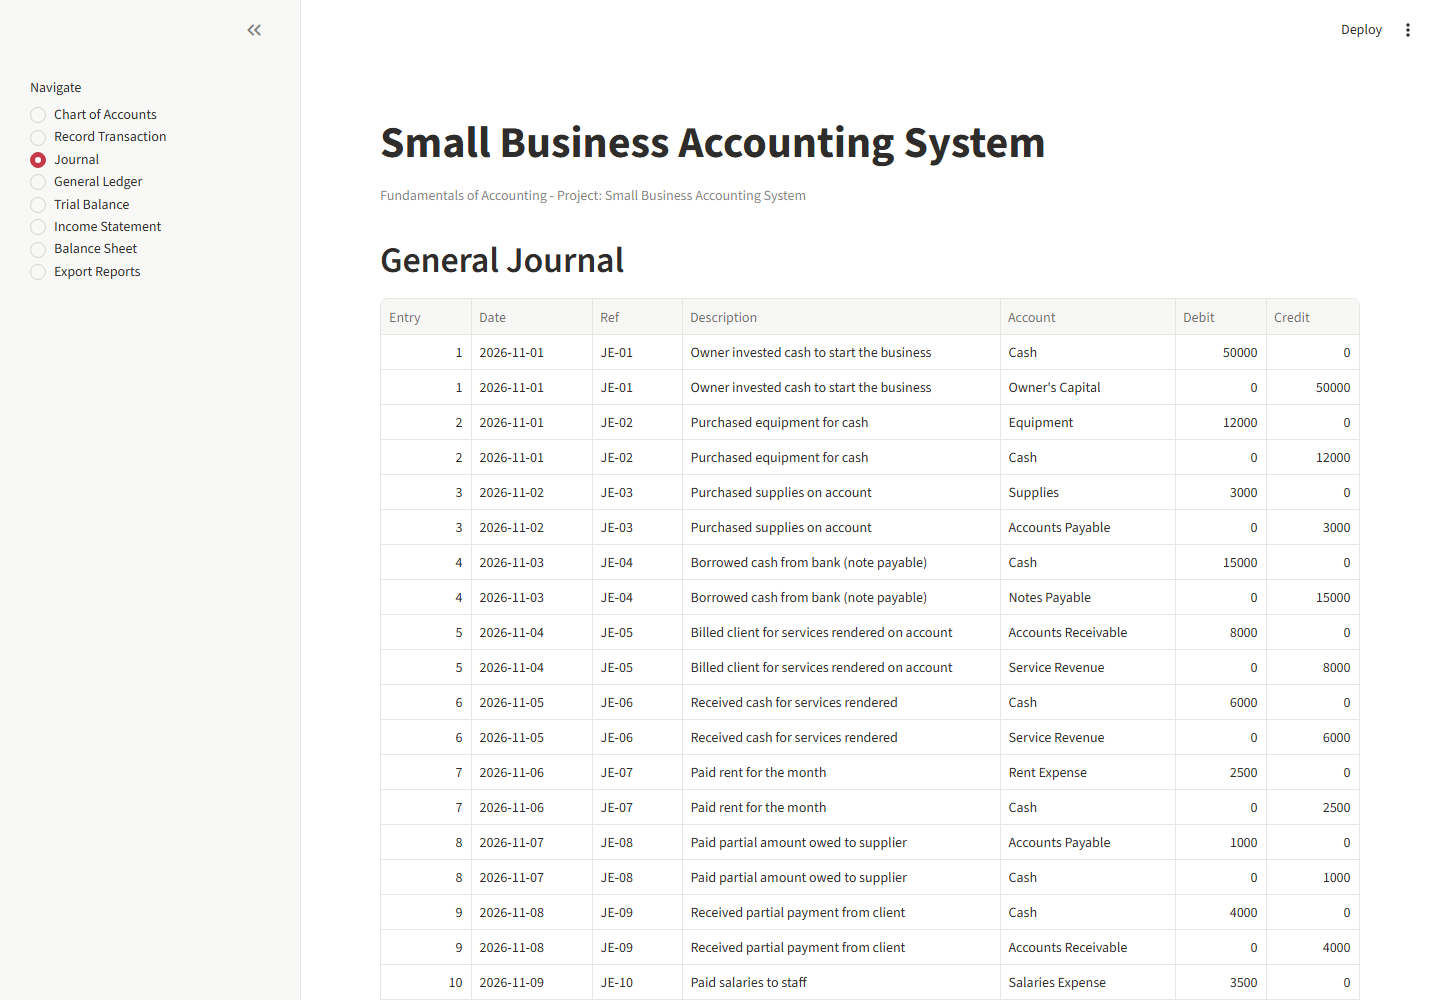
\includegraphics[width=0.85\textwidth]{../screenshots/03_journal.png}
    \caption{Full general journal listing.}
\end{figure}

\begin{figure}[h!]
    \centering
    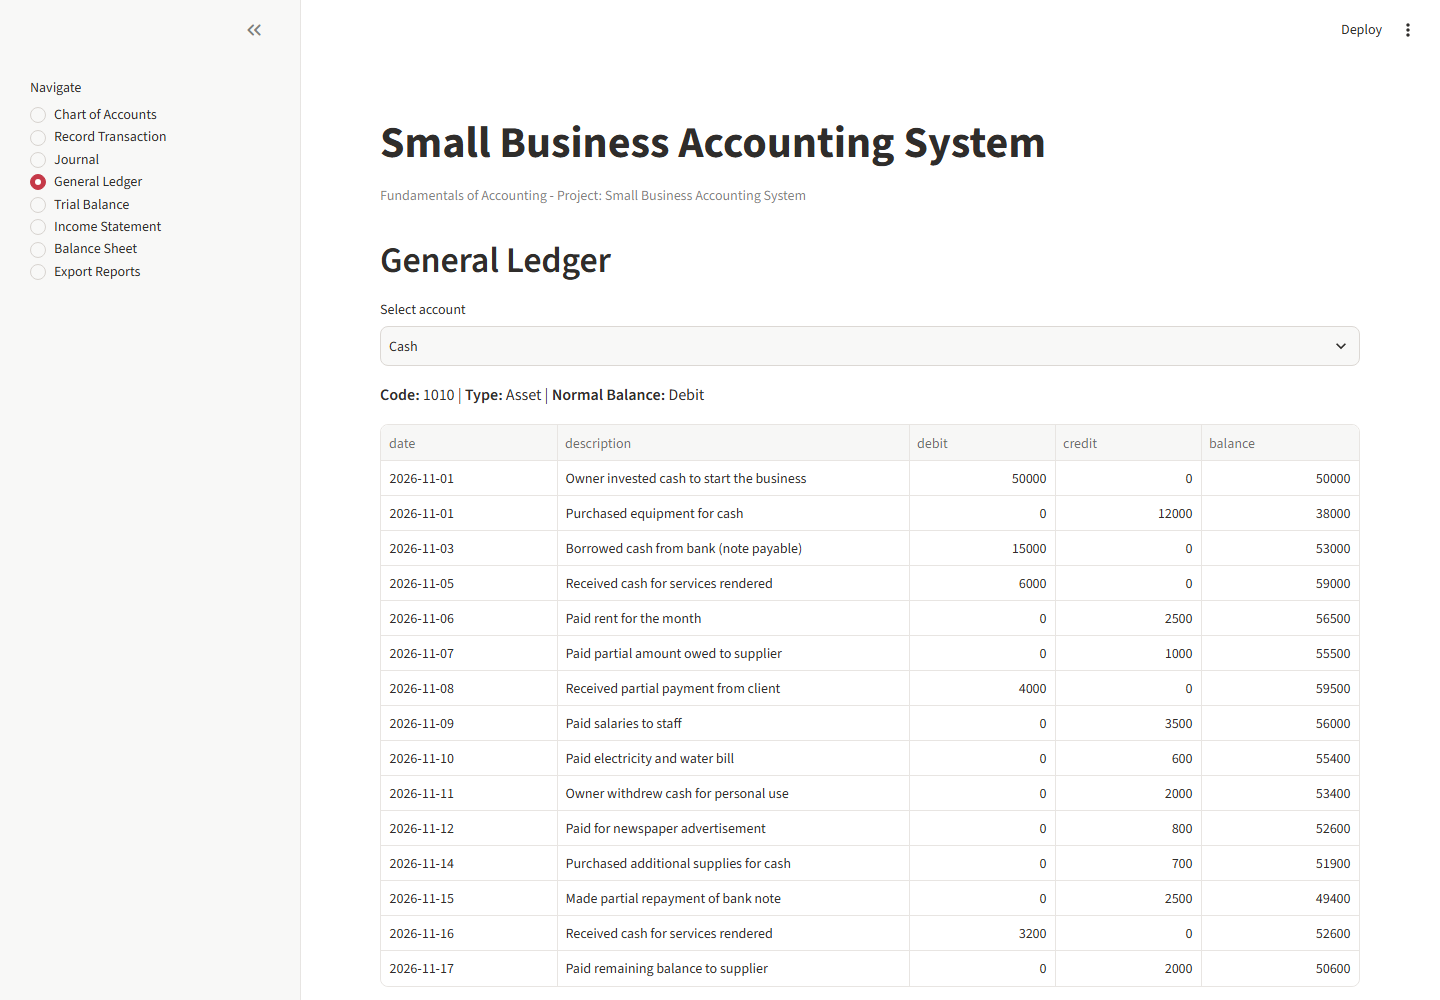
\includegraphics[width=0.85\textwidth]{../screenshots/04_general_ledger.png}
    \caption{Per-account ledger with running balance.}
\end{figure}

\begin{figure}[h!]
    \centering
    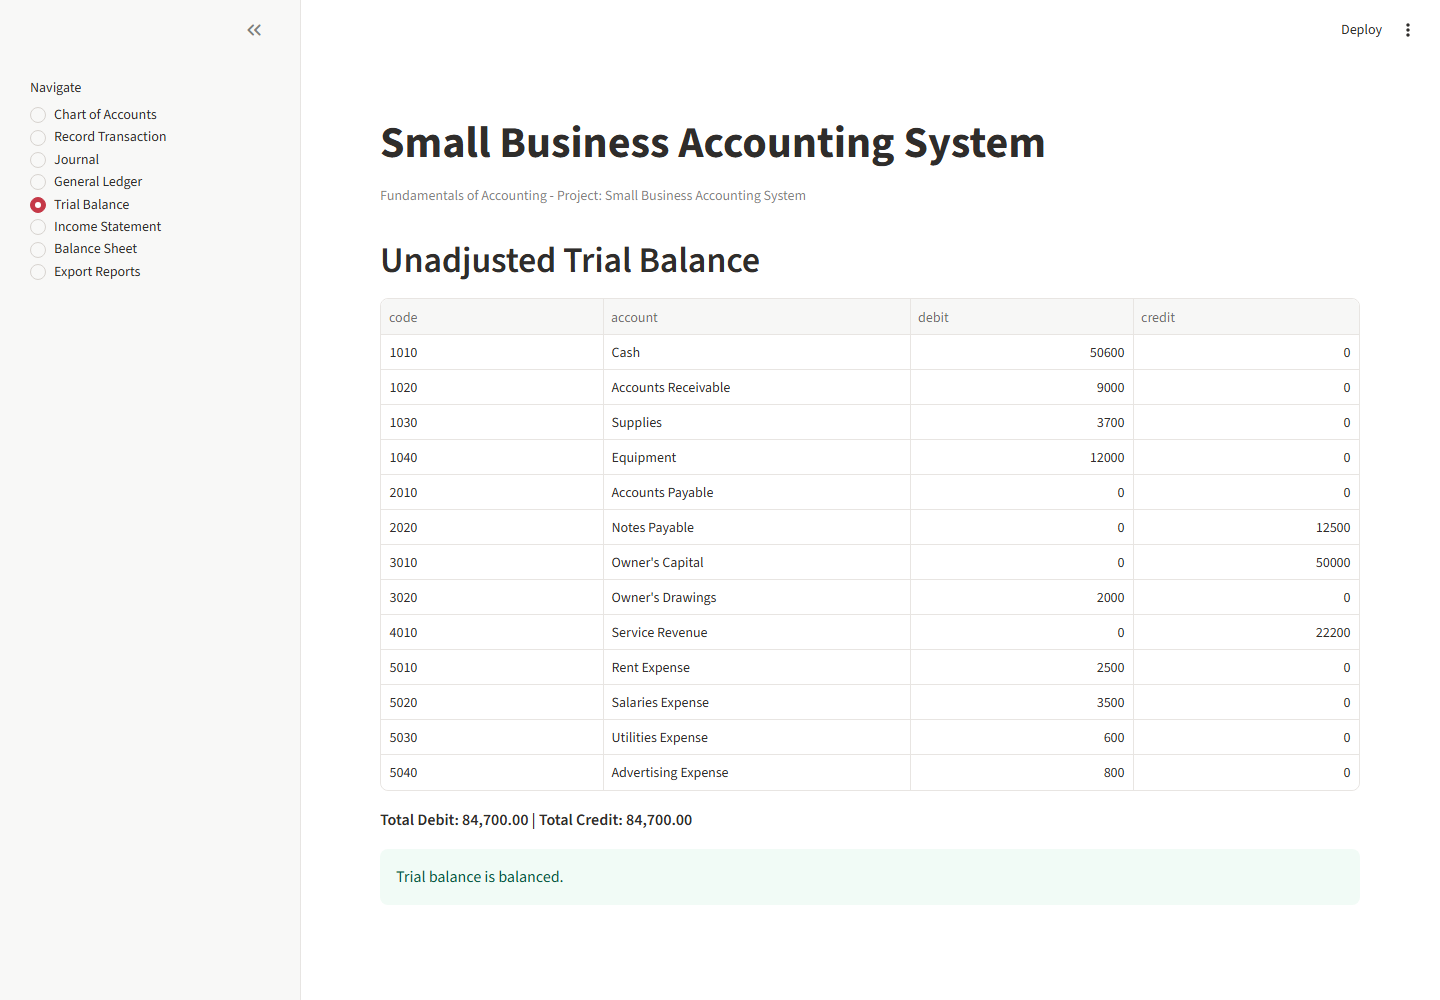
\includegraphics[width=0.85\textwidth]{../screenshots/05_trial_balance.png}
    \caption{Unadjusted trial balance, confirmed balanced (Total Debit = Total Credit = 84{,}700.00).}
\end{figure}

\begin{figure}[h!]
    \centering
    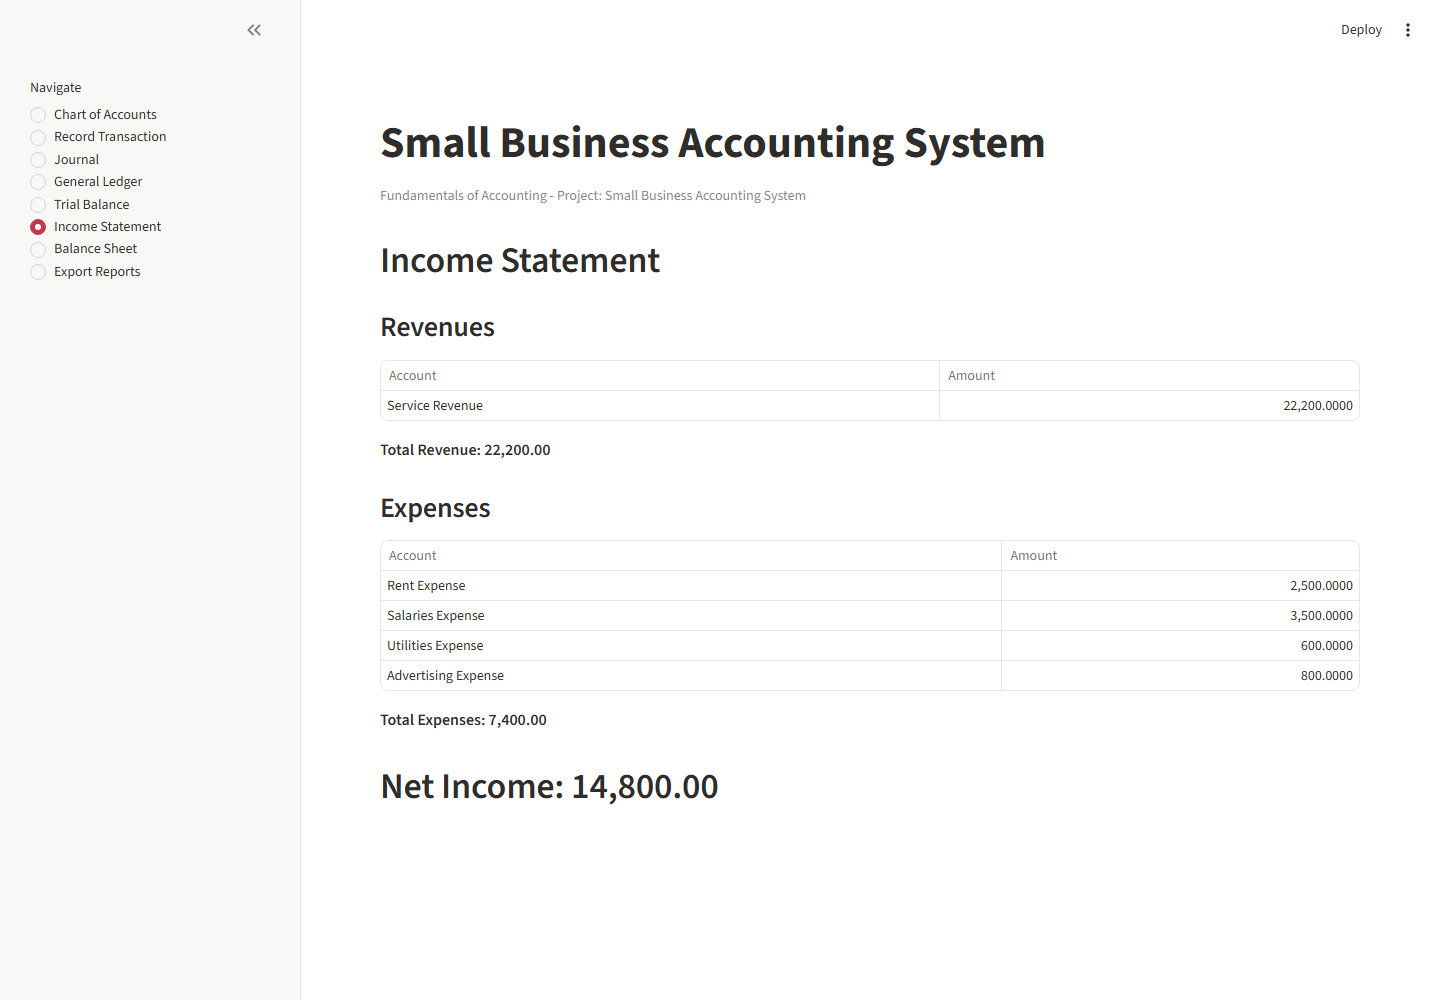
\includegraphics[width=0.85\textwidth]{../screenshots/06_income_statement.png}
    \caption{Revenues, expenses, and net income.}
\end{figure}

\begin{figure}[h!]
    \centering
    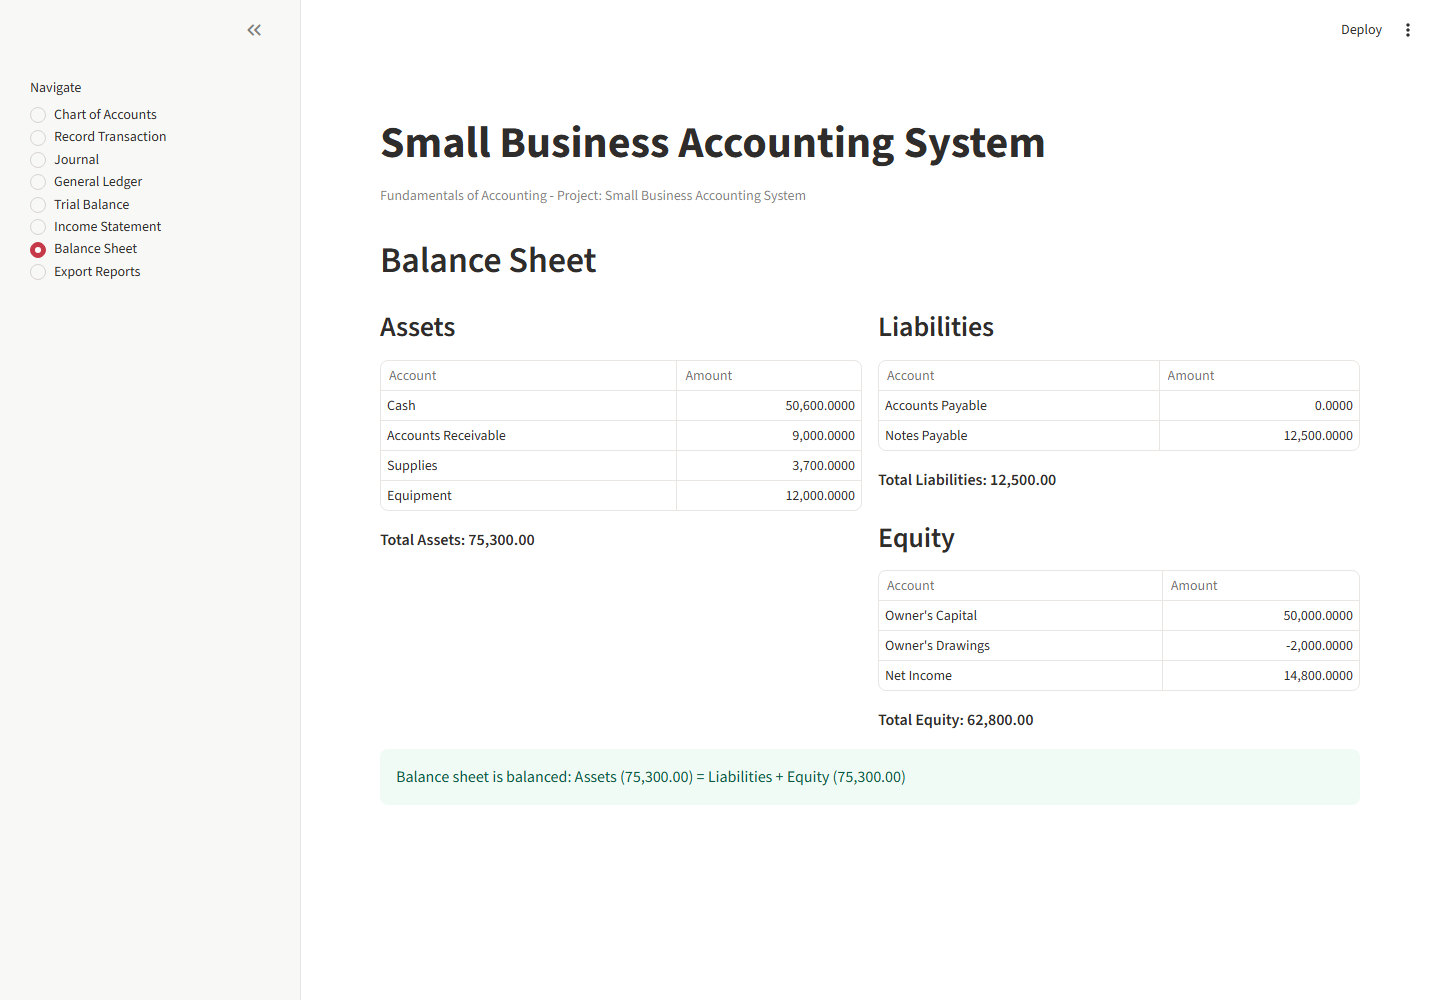
\includegraphics[width=0.85\textwidth]{../screenshots/07_balance_sheet.png}
    \caption{Assets, liabilities, equity; confirmed balanced (Assets = Liabilities + Equity = 75{,}300.00).}
\end{figure}

\begin{figure}[h!]
    \centering
    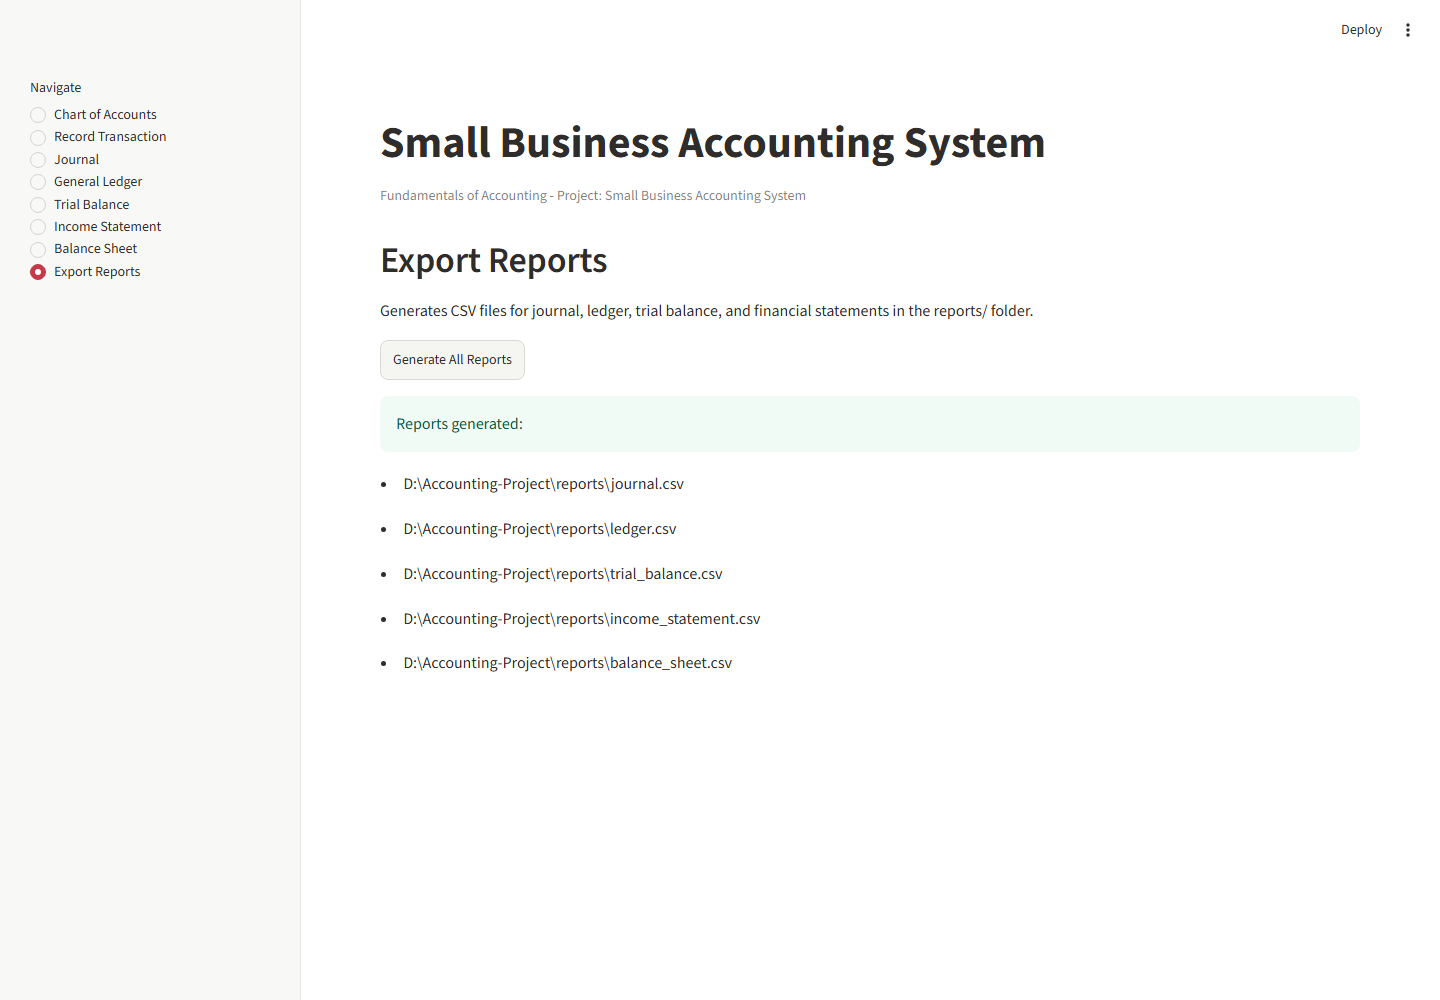
\includegraphics[width=0.85\textwidth]{../screenshots/08_export_reports.png}
    \caption{One-click CSV export of all five reports.}
\end{figure}

\begin{figure}[h!]
    \centering
    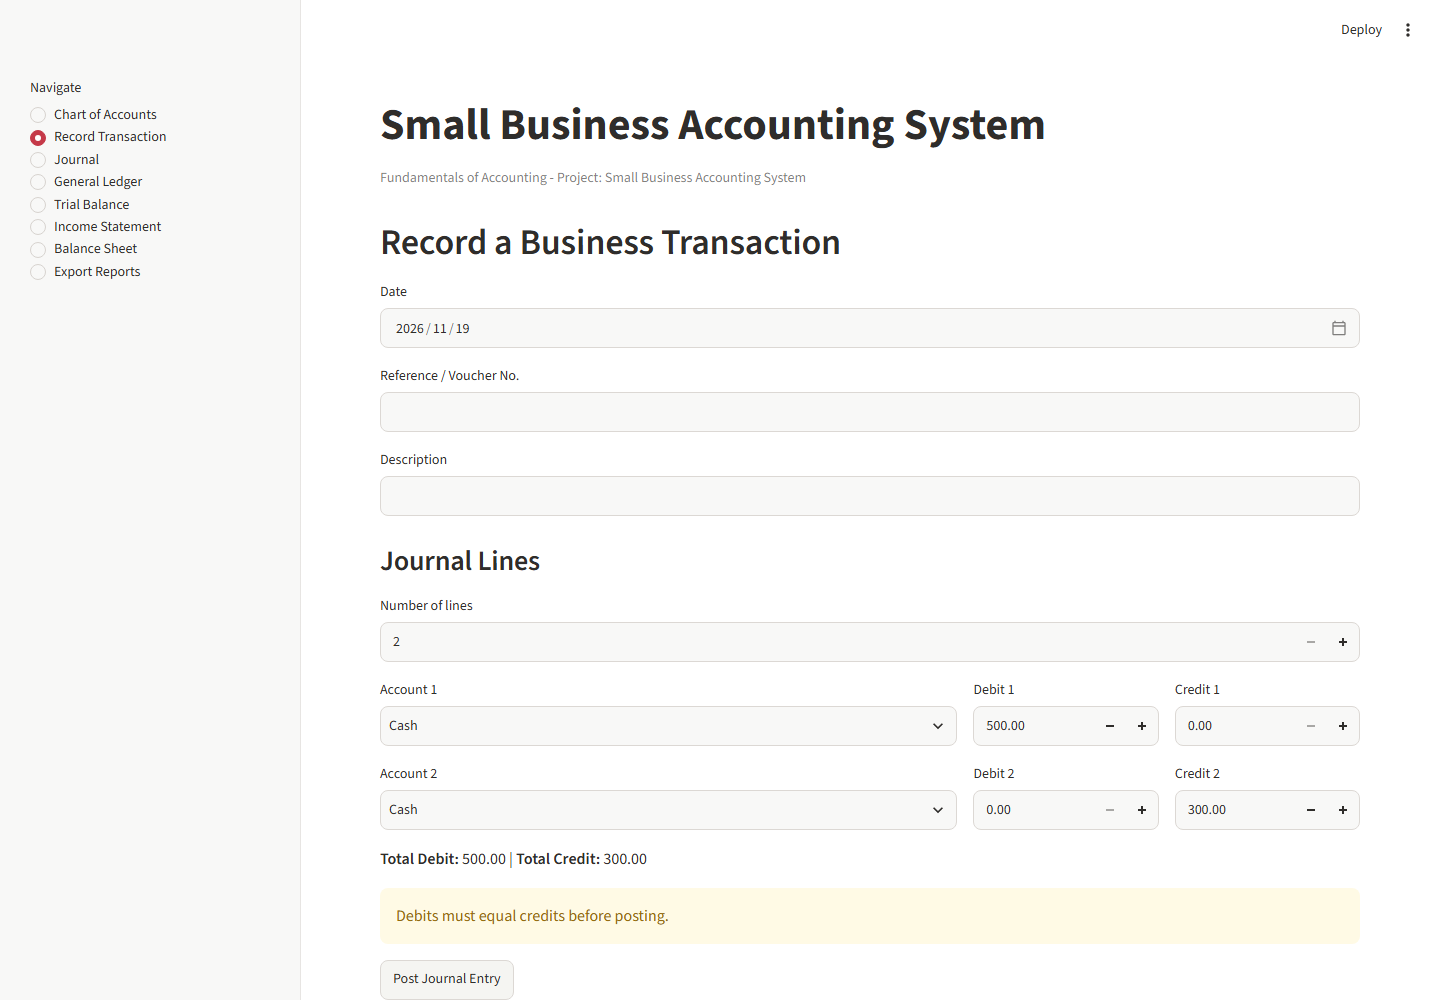
\includegraphics[width=0.85\textwidth]{../screenshots/09_validation_rejected.png}
    \caption{Unbalanced entry (Debit 500 / Credit 300) blocked with the message "Debits must equal credits before posting." (Evidence for requirement 7.)}
\end{figure}

\subsection*{Key Features}
\begin{itemize}
    \item Sidebar navigation across all 8 accounting-cycle views.
    \item Real-time balance check while entering a transaction (before posting).
    \item Server-side rejection of unbalanced entries (\texttt{UnbalancedEntryError}).
    \item Reports exportable to CSV (\texttt{reports/} folder) for printing/submission.
    \item Seed script auto-loads the 18-transaction sample dataset on first run.
\end{itemize}

% ============================================================
\section{Testing, Conclusion, and Recommendations}
% ============================================================

\subsection*{Testing Performed}

\begin{longtable}{p{3.5cm} p{4.5cm} p{5.5cm}}
\toprule
\textbf{Test} & \textbf{Method} & \textbf{Result} \\
\midrule
\endhead
Seed data loads 18 balanced transactions & \texttt{python -m app.seed} then trial balance check & Pass: Total Debit = Total Credit = 84{,}700.00 \\
Trial balance balances & \texttt{get\_trial\_balance()} & Pass: debits = credits \\
Balance sheet balances & \texttt{get\_balance\_sheet()} & Pass: Assets (75{,}300.00) = Liabilities + Equity (75{,}300.00) \\
Unbalanced entry rejected & Posted a deliberately unbalanced entry (100 debit / 50 credit) & Pass: \texttt{UnbalancedEntryError} raised, not written to DB \\
Report export & \texttt{export\_all()} & Pass: 5 CSV files generated in \texttt{reports/} \\
UI end-to-end & Streamlit app launched, all 8 pages navigated and screenshotted & Pass \\
\bottomrule
\end{longtable}

\subsection*{Conclusion}
The system satisfies all seven functional requirements in the
assignment brief: chart of accounts, $\geq$15 double-entry
transactions, journal entries, general ledger with balances, trial
balance, income statement and balance sheet, and per-entry
debit/credit validation.

\subsection*{Recommendations for Future Extension}
\begin{itemize}
    \item Add adjusting entries and a post-closing trial balance.
    \item Add multi-period support (monthly/yearly closing).
    \item Add user authentication for multi-user small-business use.
    \item Export financial statements directly to PDF.
\end{itemize}

% ============================================================
\appendix
\section{Running the Application}
% ============================================================

\begin{lstlisting}
pip install -r requirements.txt
streamlit run bookkeeping_app.py
\end{lstlisting}

App opens at \texttt{http://localhost:8501}. First run auto-seeds the
chart of accounts and 18 sample transactions into
\texttt{data/bookkeeper.db}.

To regenerate CSV reports from the command line:
\begin{lstlisting}
python -c "from app.reports import export_all; export_all()"
\end{lstlisting}

\end{document}
